\chapter{The twelve degree-of-freedom Model}
\label{chap:12dof}
\section{12DoF Model structure}
\label{sec:12dofconcept}
The model in the previous chapter is extended by integrating wheel and steering dynamics.
The additional degrees of freedom are given by wheel angular positions and (front and rear) steering angles.

Note that the additional degrees of freedom still do not allow the wheels to tilt. This means that the wheel angular velocity vectors are constrained to a horizontal plane and gyroscopic effects do not emerge.

The steering angle can no longer be an input as it is part of the vehicle state. Direction control can then only be obtained by applying steering forces.
Inputs for tyre self aligning moments are added to model the steering resistance.
Motors are modelled by inputs corresponding to the torques they generate at each wheel axle. Braking is represented by negative motor torque.
As the wheel angular velocities are included, the slip quantities are calculated within the model. The inputs and outputs are those seen in figure \ref{12flow}.
\todo{refer to block diagram in text}
\begin{figure}[ht]
  \centering
  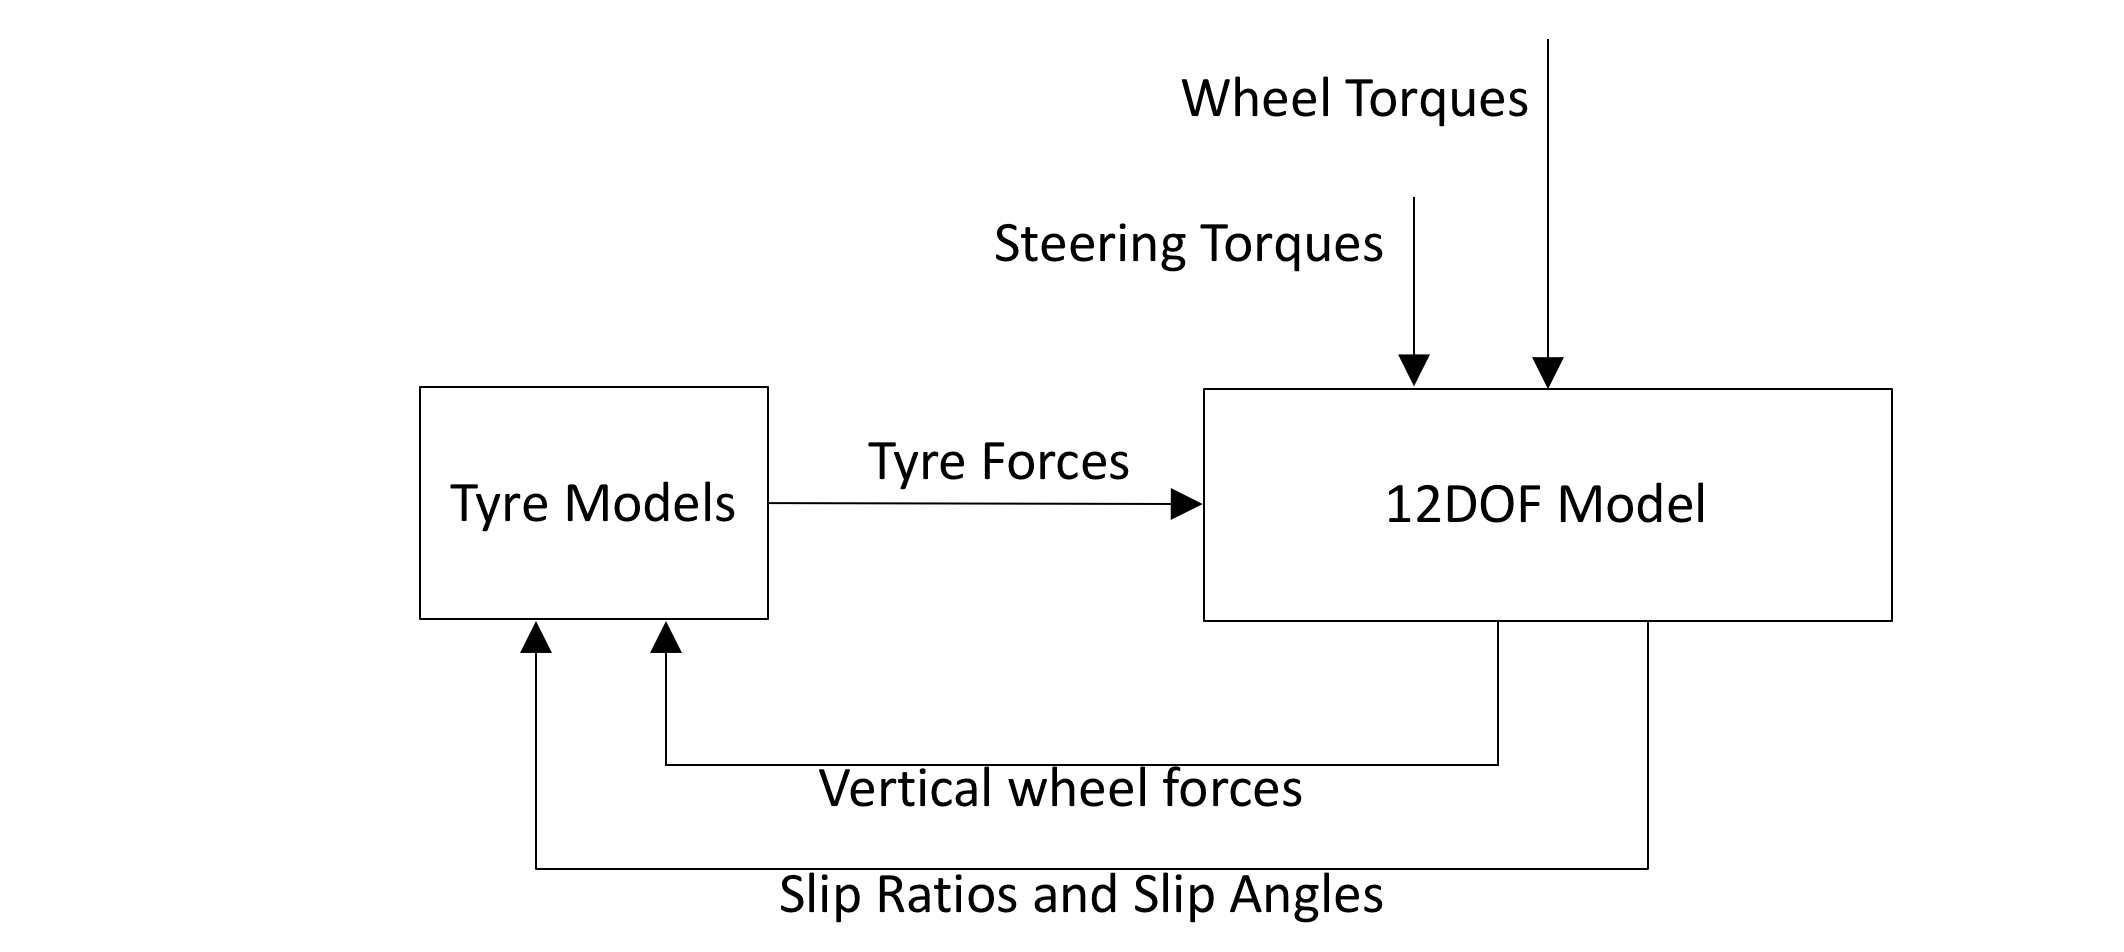
\includegraphics[width=\textwidth]{images/12flow}
  \caption{Intended Information flow for the 12 DoF Model.}
  \label{12flow}
\end{figure}

\section{Unsprung mass}
\label{sec:umass}
During the development of this second model the unsprung part of the vehicle was modelled to improve accuracy of the roll dynamics. It's mass $m_u$ was considered separately from that of the body.
The unsprung mass does not move vertically so it is not accounted for in the gravitational potential energy. The associated vertical kinetic energy is also zero.

The rotational inertia $I_u$ of the unsprung mass is also separated. The latter is a scalar because the unsprung mass only rotates around the yaw axis and does not pitch or roll.
The unsprung components weight does not act through the suspension by definition so it's contribution to the vertical wheel forces must be added separately. Assuming it is distributed equally over all four wheels the correct wheel loads are simply
$$Z'_w = Z_w + \frac{m_u}{4}g.$$

\section{Wheels}
\label{sec:wheels}
The wheels are represented by their angular positions.
The input longitudinal force on each tyre generates a moment on the wheel axis. This is summed to the motor torques and assigned to the generalized forces component associated with the corresponding wheel angular position.

Whenever the wheels are driven by the motors a reaction torque between each wheel and the chassis is generated. Each of the motor torques is expressed in vector form with respect to the inertial reference frame.

The torques are then vectorially summed. The effect of this resulting torque on the lagrangian coordinates is given by left-multiplying it with the rotational Jacobian Matrix of the chassis. The rotational Jacobian is equal to the inverse of the $E$ matrix shown in chapter \ref{chap:6dof}.

\section{Steering}
\label{sec:steering}
The wheels on each axle are assumed to be parallel to each other. The front and rear steering angles, $\delta_F$ and $\delta_R$, are defined as the angles the front and rear wheel planes form with the $xz$ plane of the undercarriage reference system.
Steering dynamics are characterized by the steering system inertia used to calculate the associated kinetic energy term in the Lagrangian.
The steering system inertias, $I_F$ and $I_R$, may be approximated by the rotational inertia of the wheel and wheel hub systems about the kingpin axes (assumed as vertical).

The steering torque inputs are summed to the self aligning tyre moment inputs and assigned to the generalized forces components associated with the corresponding steering angles.

The steering reaction to the chassis is modelled by adding the sum of the steering torques to the generalized forces component associated with the yaw angle. The rotational Jacobian can be bypassed as the steering torques act parallel to the undercarriage reference frame $z$ axis which is always coincident with yaw axis.
